\chapter{Análisis sintáctico descendente}
\section{Introducción al análisis sintáctico descendente}

Un \textit{Analizador Sintáctico Descendente} es un tipo de Analizador (ASD) que construye un árbol sintáctico de una Gramática Libre de Contexto (GLC) desde la raíz hasta las hojas. \cite{PL1}
\newline
\newline
Existen dos tipos de Analizadores ASD:
\begin{itemize}
	\item Con retroceso
	\item Sin retroceso
\end{itemize}
Básicamente un \textbf{ASD con retroceso} utiliza un método de fuerza bruta en el que trata de expandir siempre por la primera producción disponible para el símbolo no terminal más a la izquierda. Si son todos los símbolos terminales, entonces finaliza, si no, toca repetir el paso uno hasta finalizar.
\newline
\newline
Este método es muy ineficiente debido a que es probable que no se alcance la cadena del lenguaje a buscar, por lo tanto, habrá muchas vueltas atrás y producciones recursivas a la izquierda que no se pueden parar.
\newline
\newline
La \textbf{recursividad} más a la \textbf{izquierda} es un problema general de cualquier técnica de análisis sintáctico descendente por lo que tenemos que solucionar este problema, se explica más detalladamente en la sección \hyperref[sec:hello]{(5.1)}
\newline
\newline
Sin embargo, los \textbf{ASD sin retroceso} tratan de leer la cadena de izquierda a derecha, predecimos qué producción aplicar en función del símbolo o símbolos actuales de la cadena, así eliminamos las vueltas atrás, por lo que es un Análisis predictivo, tiene la peculiaridad de que solo es aplicable a un tipo especial de gramáticas, denominadas \textbf{LL(1)} y \textbf{LL(k)}.

\clearpage

\section{Gramáticas LL(1) y LL(k)}
Las gramáticas \textbf{LL(k)} son un tipo especial de gramáticas que permiten un análisis descendente sin retroceso. \cite{PL2}
\begin{itemize}
	\item L: leen la cadena de izquierda a derecha \textit{(Left to right)}
	\item L: para generar la cadena utilizan derivaciones más a la izquierda \textit{(Leftmost derivations)}
	\item k. utilizan los \textit{k} primeros símbolos de la cadena para determinar cual es la producción que se debe de aplicar.
\end{itemize}
\begin{figure}[h]
	\centering
	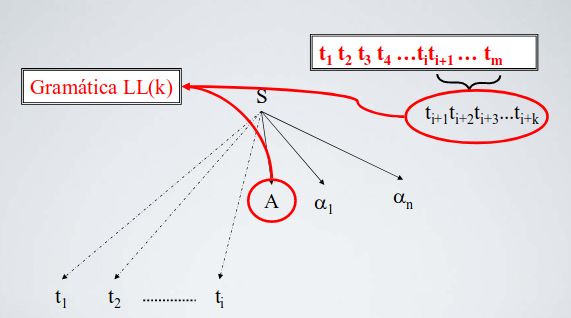
\includegraphics[width=0.5\linewidth]{img/22}
	\caption{Gramática LL(k)}
	\label{fig:2}
\end{figure}
Las gramáticas \textbf{LL(1)} son un caso particular de las gramáticas \textbf{LL(k)} en el que \textbf{k=1}
\newline
\begin{itemize}
	\item Esto quiere decir que utiliza el símbolo actual de la cadena para determinar cual es la producción que se debe de aplicar. \cite{PL2}
	
\end{itemize}

\begin{figure}[h]
	\centering
	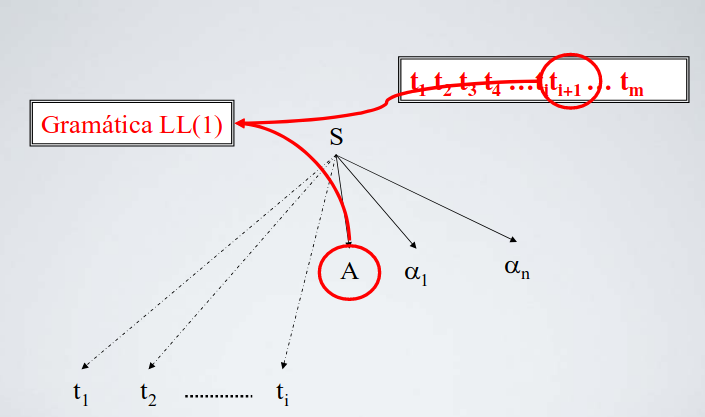
\includegraphics[width=0.5\linewidth]{img/33}
	\caption{Gramática LL(1)}
	\label{fig:4}
\end{figure}
\clearpage 

\section{Cálculo de Iniciales, Seguidores y Símbolos de predicción}
Para poder realizar el cálculo de los símbolos de predicción de nuestra gramática y poder generar nuestro \textbf{ASD} predictivo tendremos que definir la operación \textbf{Iniciales($\Upsilon$)}.
\subsection{Iniciales}
\textbf{Iniciales($\Upsilon$)} es el conjunto de símbolos terminales que pueden comenzar cualquier cadena generada por $\Upsilon$ ($\Upsilon$$\epsilon$(V$\cup$T)+)
\newline
\newline
¿Qué ocurre cuando la cadena vacía $\epsilon$ pertenece al conjunto Iniciales de alguna cadena?
\newline
Tenemos que seguir leyendo de la entrada y obtener el terminal de esa producción, o el terminal que derive del siguiente No-terminal. \cite{PL2}
\newline
\newline
\begin{figure}[h]
	\centering
	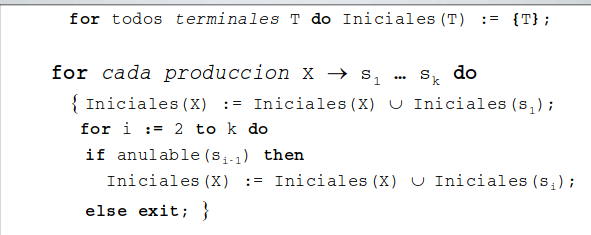
\includegraphics[width=0.7\linewidth]{img/ini}
	\caption{Cálculo iniciales}
	\label{fig:ini}
\end{figure}

Necesitamos entonces el concepto de \textbf{Anulables(X)}.
\subsubsection{Anulables}
\textbf{Anulables(X)} será igual a \textbf{True} si el No-terminal X puede generar $\epsilon$.
\begin{figure}[h]
	\centering
	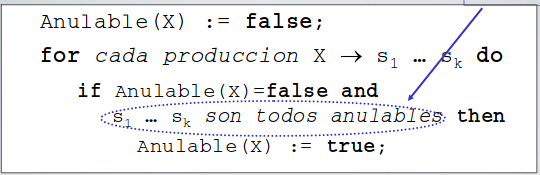
\includegraphics[width=0.7\linewidth]{img/an}
	\caption{Cálculo anulables}
	\label{fig:an}
\end{figure}
\clearpage
\subsection{Seguidores}
La operación \textbf{Seguidores(X)} calcula el conjunto de símbolos terminales t que pueden aparecer inmediatamente después del símbolo no terminal X, es decir hay una derivación desde el símbolo inicial, a una cadena con la forma $\alpha$\textbf{X}t$\beta$. \cite{PL2}

\begin{figure}[h]
	\centering
	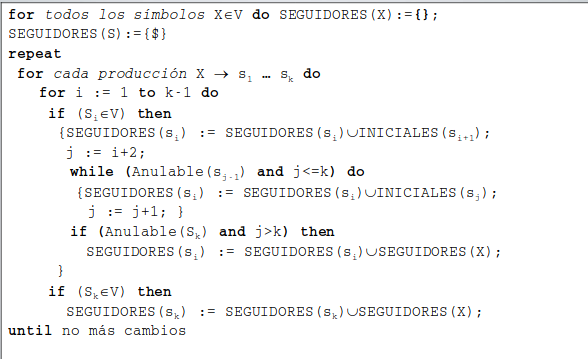
\includegraphics[width=0.7\linewidth]{img/seg}
	\caption{Calculo seguidores}
	\label{fig:seg}
\end{figure}

Esta operación que parece más compleja, realmente es sencilla, simplemente al calcular los seguidores de un No-terminal, tenemos que buscar ese No-terminal en las partes derechas de las producciones, y buscar los símbolos terminales que estén más a su derecha, y si estos fueran anulables (los No-terminales) tendríamos que calcular los iniciales del siguiente terminal o No-terminal.

\subsection{Símbolos de predicción}
Los símbolos de predicción es lo que realmente necesitamos para construir nuestro \textbf{ASD} predictivo pero para llegar hasta aquí necesitamos las operaciones anteriores.

\begin{figure}[h]
	\centering
	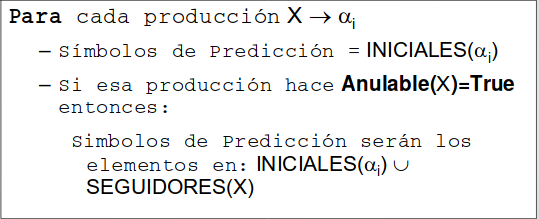
\includegraphics[width=0.7\linewidth]{img/predict}
	\caption{Cálculo de símbolos de predicción}
	\label{fig:seg}
\end{figure}

\clearpage
\section{Condición LL(1)}
\label{sec:ll1}
¿Qué propiedades ha de tener una gramática para que esta en particular sea LL(1)?
\begin{itemize}
	\item No puede ser recursiva a la izquierda
	\item Para cada producción X $\longrightarrow$ $\alpha_1$ | ... | $\alpha_k$ se tiene que cumplir que sus símbolos de predicción sean distintos, o lo que es lo mismo: \begin{itemize}
		\item  \textbf{Iniciales}($\alpha_i$) $\cap$ \textbf{Iniciales}($\alpha_j$) = $\emptyset$
		\item Si es \textbf{Anulable(X)} entonces:  \textbf{Iniciales}($\alpha_i$) $\cap$ \textbf{Seguidores}(X) = $\emptyset$
	\end{itemize}
	
\end{itemize}

\section{Gramática con recursividad por la izquierda}
\label{sec:hello}
Presentamos una gramática con el siguiente conflicto a resolver, es recursiva por la izquierda, para una mejor comprensión se utilizará la sintaxis \textbf{Proletool} \cite{Proletool} al indicar todas las gramáticas en el trabajo, pero antes ¿Qué es la recursividad por la izquierda?
\subsection{Recursividad por la izquierda}
Una gramática es \textbf{recursiva por la izquierda} cuando existe una derivación del tipo  $A \stackrel{*}{\Longrightarrow} A \alpha$
\newline
\newline
En particular, una gramática es recursiva por la izquierda si contiene una regla de producción de esa forma, en este caso la recursividad sería indirecta.
\newline
\newline
Ya sabemos que cuando la gramática es \textbf{recursiva por la izquierda} el análisis descendente predictivo no funciona, por ello tenemos que eliminarla.
\newline
\newline
\subsection{Gramática}
\begin{lstlisting}[caption = Gramática recursiva a la izquierda, style= Python]

grammar ejercicio_1{
analysis LL1;
nonterminal programa, metodo, cuerpo;
terminal class, end, def, ops, other_exp;

programa := class metodo end programa |;
metodo := metodo def | cuerpo ':';
cuerpo := ops | other_exp |;
}


\end{lstlisting}
